\documentclass[./skripsi.tex]{subfiles}
\begin{document}
\chapter{Metode Penelitian}
\section{Metode Penelitian}
\par Metode penelitian yang digunakan pada penelitian ini adalah metode penelitian kuantitatif deskriptif. Berikut adalah gambaran penelitian yang diusulkan. Berdasarkan grafik metode penelitian \ref{fig:fishbonepenelitian}, dapat dijabarkan beberapa komponen pada proses penelitian sehingga menghasilkan sebuah produk sistem yang diinginkan.
\begin{figure}%[H]
    \centering
    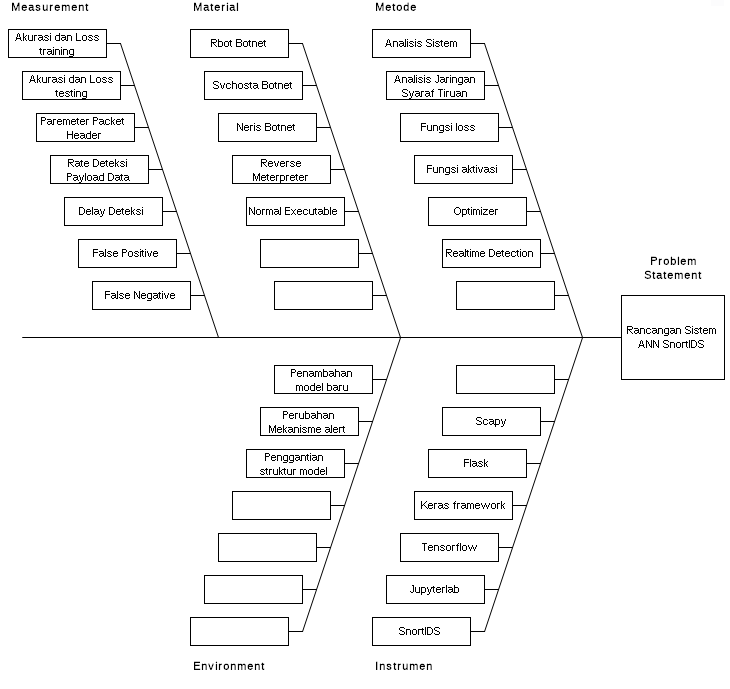
\includegraphics[width=0.8\textwidth]{public/assets/img/fishbonepenelitian.png}
    \caption{Metode Penelitian}
    \label{fig:fishbonepenelitian}
\end{figure}
\par Pada bagian \textit{measurement} menjelaskan apa saja yang dijadikan ukuran yang akan dianalisis pada penelitian ini. Parameter yang dijadikan ukuran yang akan dianalisis adalah akurasi dan loss training dan testing. Pada sistem \textit{profiling} diinputkan parameter \textit{packet header} yang dijadikan input pada LSTM. Hasil dari sistem profiling ini adalah bagaimana bentuk trafik jaringan yang akan dipelajari dan dianggap normal. Pada sistem \textit{filtering} yang dijadikan input adalah payload data, dan akan diukur hasil akurasi training dan testing pada data normal dan malicious. Pada snortIDS akan dikukur Delay Deteksi yang terjadi.
\par Pada bagian \textit{material} berisi beberapa dataset yang digunakan. Dataset yang digunakan adalah file executable windows dari botne rbot, neris, dan svchosta. Dan beberapa file tambahan seperti executable dari file exe biasa, dan virus reverse meterpreter yang digunakan untuk dijadikan tambahan pada saat testing.
\par Pada bagian \textit{environment} berisi tentang parameter kerja yang akan diubah pada sistem. Parameter ini adalah dengan menambah model pada sistem profiling yang berbeda-beda. Pada snort IDS parameter yang diubah adalah mekanisme alert pada \textit{preprocessor} nya. Dan pada proses \textit{filtering} dengan mengganti-ganti struktur model baik urutan maupun ukuran filter.
\par Pada bagian instrumen berisi tentang apa saja instrumen yang digunakan untuk memperoleh hasil penelitian. Instrumen ini antara lain \textit{scapy}, \textit{flask}, \textit{keras framework}, \textit{tensorflow}, \textit{jupyterlab}, \textit{snortIDS}. Scapy adalah \textit{library} snort yang digunakan untuk mengekstraksi data dari trafik jaringan. Flask adalah \textit{microframework} yang digunakan untuk melakukan binding model Jaringan Syaraf Tiruan. Keras sebagai framework standar dari \textit{tensorflow} digunakan untuk merancang model CNN dan LSTM.
\par Pada bagian metode berisi metode penelitian yang digunakan. Analisis sistem dilakukan untuk menjabarkan bagaiman sistem yang digunakan pada sistem \textit{filtering} dan \textit{profiling}. Analisis jaringan syaraf tiruan merupakan langkah yang dilakukan untuk menjabarkan bagaimana bentuk model jaringan syaraf tiruan yang cocok digunakan pada dataset penelitian ini. Fungsi loss, aktivasi dan optimizer merupakan parameter yang diterapkan pada model jaringan syaraf tiruan. \textit{Realtime detection} adalah metode yang digunakan untuk memperoleh delay sistem dan \textit{detection rate} pada snortIDS.
\section{Waktu dan Tempat Pelaksanaan}
\par Waktu dan tempat pelaksanaan penelitian ini adalah sebagai berikut :
\subsection{Waktu Pelaksanaan}
%Disini mulai%
%Disini selesai%
\par Waktu pelaksanaan penelitian dilakukan dari tanggal 1 Maret 2019 sampai dengan 31 Juli 2019.
\subsection{Tempat Pelaksanaan}
\par Pelaksanaan penelitian dilakukan di Laboratorium 3 UPT Pusat Teknologi Informasi dan Komunikasi Universitas Mataram
\section{Populasi dan Sampel}
\par Populasi dan sampel penelitian ini adalah sebagai berikut :
\subsection{Populasi Penelitian}
\par Populasi pada penelitian ini mencakup intrusi dalam bentuk Executable-based Virus dan Payload-based Virus
\subsection{Sampel Penelitian}
\par Sampel pada penelitian ini antara lain :
\begin{enumerate}
    \item Neris Botnet executable untuk CNN\\
    Merupakan salah satu botnet yang diperoleh dari CTU-42 dataset. Botnet ini mengirimkan data post request pada sistem C\&C channel. Payload dan executable dari botnet ini akan dijadikan sampel pada sistem \textit{filtering}
    \item Neris Botnet Traffic Data pcap untuk LSTM\\
    Berkas pcap atau \textit{packet capture} dari botnet ini dianalisis pada sistem \textit{profiling}.
    \item RBot Botnet executable untuk CNN
    Merupakan salah satu botnet yang diperoleh dari CTU-92 dataset. Botnet ini merupakan botnet lama yang menyerang sistem IRC dengan melakukan DDOS dan Spam. Payload dan executable dari botnet ini dijadikan sampel pada sistem \textit{filtering}
    \item RBot Botnet Traffic Data pcap untuk LSTM
    Berkas pcap atau \textit{packet capture} dari botnet ini dianalisis pada sistem \textit{profiling}.
    \item Svchosta Botnet executable untuk CNN\\
    Merupakan salah satu botnet yang diperoleh dari CtU-47 dataset. Botnet ini merupakan botnet yang menyerang menginfeksi file svchosta pada windows dan menyebabkan email spam, nama asli botnet ini adalah \textit{DonBot} botnet. Payload dan executable dari botnet ini akan dijadikan sampel pada sistem \textit{filtering}
    \item Svchosta Botnet Traffic Data pcap untuk LSTM
    Berkas pcap atau \textit{packet capture} dari botnet ini dianalisis pada sistem \textit{profiling}.
    \item Payload Reverse Meterpreter dalam file PE32
    \par Beberapa file executable malicious yang diselipkan dengan sengaja menggunakan \textit{metasploit framework}. Payload dan pcap dari file ini akan dijadikan bahan untuk melakukan testing pada sistem \textit{filtering} dan \textit{profiling}.
    \item File executable normal untuk CNN
    \par Beberapa file executable normal seperti firefox dan executable dari game lama windows. Payload dan pcap dari file ini akan dijadikan bahan untuk melakukan testing pada sistem \textit{filtering} dan \textit{profiling}.
\end{enumerate}
\section{Instrumen Penelitian}
Instrumen penelitian yang digunakan antara lain :
\begin{enumerate}
    \item SnortIDS sebagai Intrusion Detection System
    \item Python sebagai bahasa pemrograman yang digunakan untuk pemodelan LSTM dan CNN
    \item Library python seperti : tensorflow, keras, numpy, matplotlib untuk perlengkapan pada saat training data dan testing data dengan Convolutional Neural Network dan Long Short Term Memory.
    \item Python flask sebagai library untuk webservice filter dan profiler
    \item PC Server Linux sebagai host yang menjalankan SnortIDS, dan Python
\end{enumerate}
\subsection{Proses Pengembangan Instrumen}
\par Proses pengembangan instrumen berawal dari perancangan instrumen, uji validitas instrumen, dan uji reliabilitas instrumen.
\subsection{Uji Validitas Instrumen}
\par Proses pengujian validitas instrumen dilakukan dengan menguji IDS dengan data input yang sama, lalu mengamati hasilnya yang kemudian akan disesuaikan.
\subsection{Uji Reliabilitas Instrumen}
\par Proses pengujian reliabilitas instrumen dilakukan dengan menguji IDS dengan data input yang bervariasi ukuran datanya, dan dimuat dalam bentuk tabel \textit{detection rate}. 
\section{Prosedur Penelitian}
\par Prosedur penelitian terdiri dari perancangan sistem training dan perancangan sistem filtering dan profiling untuk testing. Rancangan sistem training dibuat dengan menggunakan jupyter notebook. Sedangkan rancangan sistem filter menggunakan snortIDS dan flask framework untuk menghubungkan keluaran data dari snortIDS ke dalam model CNN dan LSTM.
\subsection{Perancangan Sistem}
\begin{figure}
    \centering
    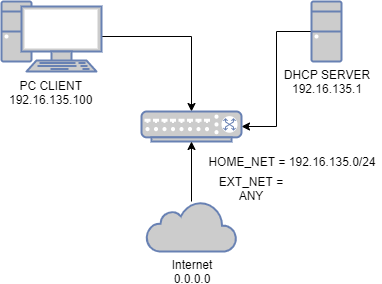
\includegraphics[width=0.5\textwidth]{public/assets/img/Topologi.png}
    \caption{Topologi jaringan}
    \label{fig:topologi_jaringan}
\end{figure}
\par Sistem preprocessor diterapkan pada topologi jaringan seperti pada gambar \ref{fig:topologi_jaringan}. Seluruh proses dilakukan pada sisi PC Client. Ketika PC Client mendownload data dari internet atau PC lain mengupload data ke PC Client, PC Client akan melakukan proses filter dan profiling, kemudian menentukan bahwa data yang dikirim aman atau tidak.
\par Rancangan sistem filter terdiri dari Dataset yang dijadikan data untuk proses testing. Pada sisi filter juga terdapat IP\_buffer yang digunakan sebagai input yang akan mengumpulkan packet yang bersumber dari alamat IP yang sama.

\begin{figure}%[H]
    \centering
    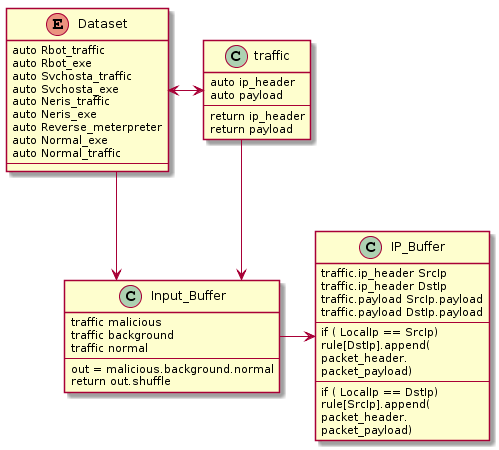
\includegraphics[width=0.9\textwidth]{public/assets/img/RancanganSistemPenelitian.png}
    \caption{Model Rancangan Sistem}
    \label{fig:rancanganpenelitian}
\end{figure}

\par Berdasarkan gambar \ref{fig:rancanganpenelitian}, dapat dijabarkan rancangan sistem yang akan dibuat untuk \textit{preprocessor} terdiri dari sistem \textit{profiling} dengan metode LSTM dan sistem \textit{filtering} dengan metode CNN.

\par Dari gambar \ref{fig:rancanganpenelitian} juga dapat dijelaskan bahwa dataset yang digunakan adalah beberapa \textit{botnet}, \textit{reverse meterpreter}, dan \textit{file executable normal}. Kemudian dari beberapa file ini akan diambil bagian-bagian yang akan dijadikan analisa yakni bagian \textit{header} dan bagian \textit{payload} nya. Sebelum dapat diproses oleh sistem, semua isi packet ini di masukkan ke dalam input buffer untuk kemudian dilanjutkan. Untuk di proses oleh sistem.

\begin{figure}%[H]
    \centering
    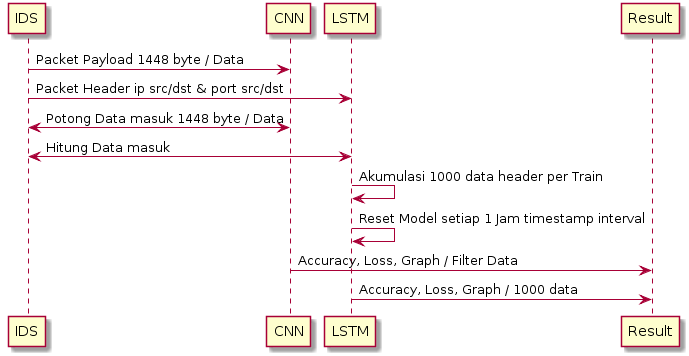
\includegraphics[width=0.9\textwidth]{public/assets/img/sistemtransaksicnnlstm.png}
    \caption{Proses kerja sistem training}
    \label{fig:proseskerjasistem}
\end{figure}

\par Berdasarkan gambar \ref{fig:proseskerjasistem}, dapat dijabarkan proses kerja sistem yang akan dirancang. Rancangan sistem untuk mendapatkan hasil diperoleh dari IDS sebagai sistem pendeteksi intrusi, CNN sebagai sistem \textit{filtering}, dan LSTM sebagai sistem \textit{filtering}

\begin{figure}%[H]
    \centering
    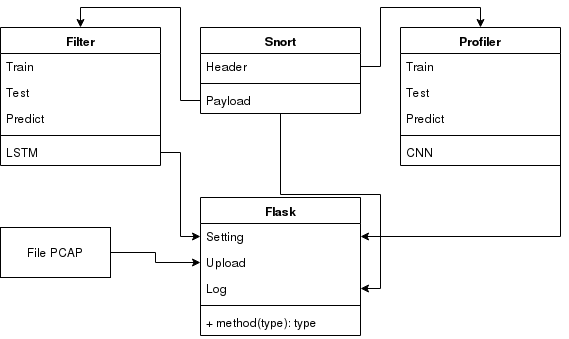
\includegraphics[width=0.9\textwidth]{public/assets/img/SistemTA.png}
    \caption{Proses Kerja sistem}
    \label{fig:proseskerja}
\end{figure}
\par Berdasarkan gambar \ref{fig:proseskerja} dapat dijabarkan rancangan sistem inti terdiri dari snort, filter, dan profiler,  dengan tampilan menggunakan flask. Pemroresan data dan analisis data terjadi pada sistem snort, LSTM dan CNN, yang kemudian hasilnya akan diteruskan menjadi grafik dan ditampilkan dengan flask.
\section{Analisis Data}
\par Proses analisis data meliputi analisis tabel dan analisis grafis dari seluruh hasil pengujian validitas dan reliabilitas instrumen
\subsection{Prosedur Pengolahan Data}
\par Sebelum data dimasukkan, data yang masih mentah diubah menjadi data angka. Pada sistem \textit{profiling}, data angka yang dijadikan input adalah data header yang berisi \textit{IP Address}, \textit{Port} baik sumber maupun tujuan dan beberapa parameter header lainnya. Pada sistem \textit{filtering}, data angka yang dijadikan input diperoleh dari data 1448 byte per frame packet yang diperoleh dari \textit{packet payload}.
\par Setelah diperoleh data angka pada sistem \textit{profiling} di inputkan data angka header, lalu proses \textit{training} dilakukan untuk memperoleh hasil regresi dari trafik jaringan. Sedangkan pada sistem \textit{filtering} di inputkan data payload yang kemudian akan di lakukan training untuk mengklasifikasi data yang dimasukkan aman atau intrusi. Data hasil training dan testing dari proses ini akan dianalisis untuk menentukan model yang akan digunakan pada sistem pendeteksi intrusi SnortIDS.
\par Setelah diperoleh model yang sesuai diperoleh. Model yang sudah jadi dibinding oleh \textit{flask} dan dapat diakses dengan HTTP Request. Data hasil keluaran snortIDS akan dikirim ke \textit{flask} ini untuk dilakukan analisis dan diperoleh hasil prediksinya. Dari proses ini diperoleh delay sistem dan \textit{detection rate} dari kinerja snortIDS.
\subsubsection{Proses Parsing Paket Jaringan}
\par Sebelum data dapat diolah, sebelumnya data mentah pcap harus melalui ekstraksi header dan payload. Diketahui struktur data PCAP adalah sebagai berikut.
\begin{figure}%[H]
\centering
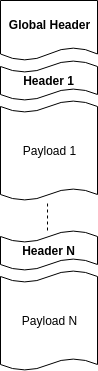
\includegraphics[width=0.35\textwidth]{public/assets/img/PCAPStruktur.png}
\caption{Struktur Data File PCAP}
\label{fig:pcapstruktur}
\end{figure}

\par Dapat dilihat pada gambar \ref{fig:pcapstruktur}, file pcap terdiri dari sebuah Global Header dan beberapa \textit{Packet Header} dan \textit{Packet Payload}.
\begin{figure}%[H]
\centering
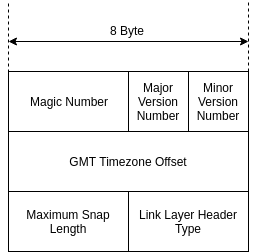
\includegraphics[width=0.5\textwidth]{public/assets/img/GlobalHeader.png}
\caption{Global Header}
\label{fig:globalheader}
\end{figure}
\par Berdasarkan gambar \ref{fig:globalheader} dapat diamati \textit{Global Header} terdiri dari 4 byte \textit{Magic Number} yakni D4 C3 B2 A1 yang menandakan jenis file PCAP. Kemudian diikuti dengan 4 byte \textit{Version Number} yang merupakan versi dari file PCAP. Kemudian 8 byte berikutnya berisi timezone offset berdasarkan lokasi dari file PCAP diambil. Kemudian 4 byte selanjutnya berisi \textit{Maximum Snap Length} yang berisi tentang ukuran maksimum frame setiap packet yang diambil. Kemudian 4 byte selanjutnya berisi  \textit{Link Layer Header Type} yang berisi informasi tentang link layer yang digunakan.
\par Beberapa header yang umum pada \textit{Packet Header} antara lain :
\begin{figure}%[H]
    \centering
    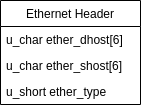
\includegraphics[width=0.3\textwidth]{public/assets/img/EthernetHeader.png}
    \caption{Ethernet Header}
    \label{fig:ethernetheader}
\end{figure}
\par Ethernet Header dijelaskan pada gambar \ref{fig:ethernetheader}, header ini berisi informasi MAC Address pengirim dan penerima. Header ini berukuran 14 byte yang terdiri dari ether\_dhost sebesar 6 byte, ether\_shost sebesar 6 byte, dan ether\_type sebesar 2 byte.
\begin{figure}%[H]
    \centering
    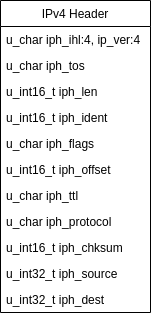
\includegraphics[width=0.3\textwidth]{public/assets/img/IPV4Header.png}
    \caption{IPV4 Header}
    \label{fig:ipv4header}
\end{figure}
\par IPv4 Header dijelaskan pada gambar \ref{fig:ipv4header}, header ini berisi informasi tentang alamat IP sumber dan tujuan. Header ini berukuran 20 byte yang terdiri dari 1 byte iph\_ihl dan iph\_ver, 1 byte iph\_tos, 2 byte iph\_len, 2 byte iph\_indent, 1 byte iph\_flags, 2 byte iph\_offset, 1 byte iph\_ttl, 1 byte iph\_protocol, 2 byte iph\_chksum, 4 byte iph\_source, 4 byte iph\_dhost.
\begin{figure}%[H]
    \centering
    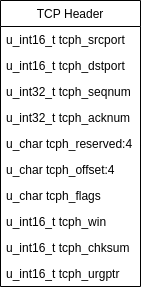
\includegraphics[width=0.3\textwidth]{public/assets/img/TCPHeader.png}
    \caption{TCP Header}
    \label{fig:tcpheader}
\end{figure}
\par TCP Header memiliki struktur sesuai dengan gambar \ref{fig:tcpheader}, header ini berisi tentang informasi port sumber dan tujuan. Header ini berukuran 20 byte yang terdiri dari 2 byte tcph\_srcport, 2 byte tcph\_dstport, 4 byte tcph\_seqnum, 4 byte tcph\_acknum, 1 byte tcph\_reserved dan tcph\_offset, 1 byte tcph\_flags, 2 byte tcph\_win, 2 byte tcph\_chksum, 2 byte tcph\_urgptr.
\begin{figure}%[H]
    \centering
    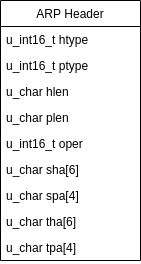
\includegraphics[width=0.3\textwidth]{public/assets/img/ARPHeader.png}
    \caption{ARP Header}
    \label{fig:arpheader}
\end{figure}
\par ARP Header memiliki struktur data sesuai dengan gambar \ref{fig:arpheader}, header ini berisi tentang informasi tentang \textit{Address Resolution Protocol}. Header ini berukuran 28 byte yang terdiri dari 2 byte htype, 2 byte ptype, 1 byte hlen, 1 byte plen, 2 byte operation, 6 byte sha, 4 byte spa, 6 byte tha, 4 byte tpa.
\begin{figure}%[H]
    \centering
    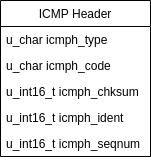
\includegraphics[width=0.3\textwidth]{public/assets/img/ICMPHeader.png}
    \caption{ICMP Header}
    \label{fig:icmpheader}
\end{figure}
\par ICMP (\textit{Internet Control Message Protocol}) Header memiliki struktur data pada gambar \ref{fig:icmpheader}, header ini berisi tentang informasi \textit{Control Message} yang dikeluarkan oleh program seperti Ping ataupun Traceroute. Header ini berukuran 8 byte terdiri dari 1 byte icmph\_type, 1 byte icmph\_code, 2 byte icmph\_chksum, 2 byte icmph\_ident, 2 byte icmph\_seqnum.
\par Beberapa jenis packet terdiri dari beberapa header, contohnya adalah ARP Packet, ICMP Packet, UDP Packet, TCP Packet, dan HTTP Packet yang merupakan bahan analisis pada penelitian ini.
\begin{figure}%[H]
    \centering
    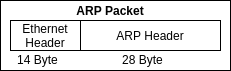
\includegraphics[height=2cm]{public/assets/img/ARPPacket.png}
    \caption{ARP Packet}
    \label{fig:arppaket}
\end{figure}
\par Gambar \ref{fig:arppaket} menunujukkan bahwa ARP Packet hanya terdiri dari Ethernet Header yang berukuran 14 byte, dan ARP Header 28 byte.
\begin{figure}%[H]
    \centering
    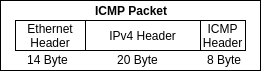
\includegraphics[height=2cm]{public/assets/img/ICMPPacket.png}
    \caption{ICMP Packet}
    \label{fig:icmppaket}
\end{figure}
\par Dari gambar \ref{fig:icmppaket} dapat diamati bahwa ICMP Packet terdiri dari Ethernet Header yang berukuran 14 byte, IPV4 Header yang berukuran 20 byte, dan ICMP Header yang berukuran 8 byte.
\begin{figure}%[H]
    \centering
    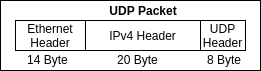
\includegraphics[height=2cm]{public/assets/img/UDPPacket.png}
    \caption{UDP Packet}
    \label{fig:udppaket}
\end{figure}
\par Dapat diamati pada gambar \ref{fig:udppaket}, UDP Packet terdiri atas 14 byte Ethernet Header, 20 byte IPv4 Header, dan 8 byte UDP Header.
\begin{figure}%[H]
    \centering
    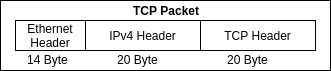
\includegraphics[height=2cm]{public/assets/img/TCPPacket.png}
    \caption{TCP Packet}
    \label{fig:tcppaket}
\end{figure}
\par Gambar \ref{fig:tcppaket} menjabarkan bahwa TCP Packet terdiri atas 14 byte Ethernet Header, 20 byte IPv4 Header, dan 20 byte TCP Header.
\begin{figure}%[H]
    \centering
    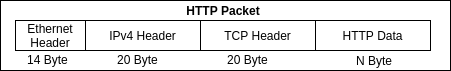
\includegraphics[height=2cm]{public/assets/img/HTTPPacket.png}
    \caption{HTTP Packet}
    \label{fig:httppaket}
\end{figure}
\par Dapat diamati dari gambar \ref{fig:httppaket} bahwa HTTP Paket merupakan TCP Paket yang memiliki data HTTP di dalamnya. Data ini yang kemudian akan dijadikan bahan analisa pada penelitian ini sebagai payload.
\subsection{Teknik Analisis Data}
\par Analisis data dilakukan berdasarkan dua jenis data yang diperoleh yakni Sistem \textit{Profiling} oleh LSTM, dan Sisitem \textit{Filtering} oleh CNN. Sistem Profiling LSTM menggunakan tiga metode yakni \textit{Sentiment Analysis}, \textit{Multivariate Prediction}, dan \textit{4 Directional Header Prediction}. Ketiga metode ini kemudian masing-masing parameternya akan di analisis agar memperoleh Sistem \textit{Profiling} yang optimal. Sistem Filtering CNN dianalisis dengan mengubah parameter \textit{learning rate}-nya. Dimana \textit{learning rate} yang dipakai adalah 0.1, 0.01, 0.001, dan 0.0001. Hal ini dilakukan untuk mempertimbangkan learning rate yang optimal yang akan digunakan untuk melakukan training model filter.
\par Untuk menguji analisis payload CNN pada jenis data yang berbeda maka diperlukan beberapa tambahan data lain. Pada analisis data CNN diberikan payload tambahan yakni file executable yang berisi reverse meterpreter, dan file executable sebelum diisikan reverse meterpreter. Berikut ini adalah daftar file executable yang digunakan sebagai tambahan :
\begin{table}%[H]
\centering
\begin{tabularx}{0.5\textwidth}{|l|X|}
\hline
\textbf{Nama Program} & \textbf{Nama File} \\
\hline
Calculator & calc.exe\\
\hline
Cruel game & cruel.exe\\
\hline
Freecell game & freecell.exe\\
\hline
Golf game & golf.exe\\
\hline
MS Paint & mspaint.exe\\
\hline
Pegged & pegged.exe\\
\hline
Realterm & realterm.exe\\
\hline
Reversi game & reversi.exe\\
\hline
Snake game & snake.exe\\
\hline
Solitaire game & sol.exe\\
\hline
Taipei game & taipei.exe\\
\hline
Winmine game & winmine.exe\\
\hline
\end{tabularx}
\caption{Dataset tambahan}
\label{table:dataset_tambahan}
\end{table}
\par Dapat diamati pada tabel \ref{table:dataset_tambahan}, sebagian besar file executable adalah file dengan jenis executable windows. Hal ini dilakukan untuk mempermudah memasukkan data reverse meterpreter dalam file tersebut.
\subsection{Membuat klasifikasi data}
\par Data kelas terbagi menjadi 2 yakni \textit{Malicious} dan \textit{Benign}. Untuk membedakan kedua kelas ini dilakukan training pada data \textit{malicious} dengan dua kelas. Pada sistem filtering klasifikasi terjadi berdasarkan sifat dari payload dari \textit{packet}, sedangkan pada sistem profiling klasifikasi terjadi secara tidak langsung, dengan memperhitungkan anomali trafik jaringan dengan regresi.
\end{document}
